\let\negmedspace\undefined
\let\negthickspace\undefined
\documentclass[journal,12pt,twocolumn]{IEEEtran}
\usepackage{gensymb}
\usepackage{amssymb}
\usepackage[cmex10]{amsmath}
\usepackage{amsthm}
\usepackage[export]{adjustbox}
\usepackage{bm}
\usepackage{longtable}
\usepackage{enumitem}
\usepackage{mathtools}
 \usepackage{tikz}
\usepackage[breaklinks=true]{hyperref}
\usepackage{listings}
\usepackage{color}                                            %%
\usepackage{array}                                            %%
\usepackage{longtable}                                        %%
\usepackage{calc}                                             %%
\usepackage{multirow}                                         %%
\usepackage{hhline}                                           %%
\usepackage{ifthen}                                           %%
\usepackage{lscape}     
\usepackage{multicol}
% \usepackage{enumerate}
\DeclareMathOperator*{\Res}{Res}
\renewcommand\thesection{\arabic{section}}
\renewcommand\thesubsection{\thesection.\arabic{subsection}}
\renewcommand\thesubsubsection{\thesubsection.\arabic{subsubsection}}
\renewcommand\thesectiondis{\arabic{section}}
\renewcommand\thesubsectiondis{\thesectiondis.\arabic{subsection}}
\renewcommand\thesubsubsectiondis{\thesubsectiondis.\arabic{subsubsection}}
\hyphenation{op-tical net-works semi-conduc-tor}
\def\inputGnumericTable{}                                 %%
\lstset{
frame=single, 
breaklines=true,
columns=fullflexible
}
\begin{document}
\newcommand{\BEQA}{\begin{eqnarray}}
\newcommand{\EEQA}{\end{eqnarray}}
\newcommand{\define}{\stackrel{\triangle}{=}}
\newcommand*\circled[1]{\tikz[baseline=(char.base)]{
    \node[shape=circle,draw,inner sep=2pt] (char) {#1};}}
\bibliographystyle{IEEEtran}
\providecommand{\mbf}{\mathbf}
\providecommand{\pr}[1]{\ensuremath{\Pr\left(#1\right)}}
\providecommand{\qfunc}[1]{\ensuremath{Q\left(#1\right)}}
\providecommand{\sbrak}[1]{\ensuremath{{}\left[#1\right]}}
\providecommand{\lsbrak}[1]{\ensuremath{{}\left[#1\right.}}
\providecommand{\rsbrak}[1]{\ensuremath{{}\left.#1\right]}}
\providecommand{\brak}[1]{\ensuremath{\left(#1\right)}}
\providecommand{\lbrak}[1]{\ensuremath{\left(#1\right.}}
\providecommand{\rbrak}[1]{\ensuremath{\left.#1\right)}}
\providecommand{\cbrak}[1]{\ensuremath{\left\{#1\right\}}}
\providecommand{\lcbrak}[1]{\ensuremath{\left\{#1\right.}}
\providecommand{\rcbrak}[1]{\ensuremath{\left.#1\right\}}}
\theoremstyle{remark}
\newtheorem{rem}{Remark}
\newcommand{\sgn}{\mathop{\mathrm{sgn}}}
\providecommand{\abs}[1]{\left\vert#1\right\vert}
\providecommand{\res}[1]{\Res\displaylimits_{#1}} 
\providecommand{\norm}[1]{\left\lVert#1\right\rVert}
%\providecommand{\norm}[1]{\lVert#1\rVert}
\providecommand{\mtx}[1]{\mathbf{#1}}
\providecommand{\mean}[1]{E\left[ #1 \right]}
\providecommand{\fourier}{\overset{\mathcal{F}}{ \rightleftharpoons}}
%\providecommand{\hilbert}{\overset{\mathcal{H}}{ \rightleftharpoons}}
\providecommand{\system}{\overset{\mathcal{H}}{ \longleftrightarrow}}
	%\newcommand{\solution}[2]{\textbf{Solution:}{#1}}
\newcommand{\solution}{\noindent \textbf{Solution: }}
\newcommand{\cosec}{\,\text{cosec}\,}
\providecommand{\dec}[2]{\ensuremath{\overset{#1}{\underset{#2}{\gtrless}}}}
\newcommand{\myvec}[1]{\ensuremath{\begin{pmatrix}#1\end{pmatrix}}}
\newcommand{\mydet}[1]{\ensuremath{\begin{vmatrix}#1\end{vmatrix}}}
\newcommand*{\permcomb}[4][0mu]{{{}^{#3}\mkern#1#2_{#4}}}
\newcommand*{\perm}[1][-3mu]{\permcomb[#1]{P}}
\newcommand*{\comb}[1][-1mu]{\permcomb[#1]{C}}
%\numberwithin{equation}{subsection}
\makeatletter
\@addtoreset{figure}{problem}
\makeatother
\let\StandardTheFigure\thefigure
\let\vec\mathbf
\renewcommand{\thefigure}{\theproblem}
\def\putbox#1#2#3{\makebox[0in][l]{\makebox[#1][l]{}\raisebox{\baselineskip}[0in][0in]{\raisebox{#2}[0in][0in]{#3}}}}
     \def\rightbox#1{\makebox[0in][r]{#1}}
     \def\centbox#1{\makebox[0in]{#1}}
     \def\topbox#1{\raisebox{-\baselineskip}[0in][0in]{#1}}
     \def\midbox#1{\raisebox{-0.5\baselineskip}[0in][0in]{#1}}
\vspace{3cm}
\title{Assignment-2}
\author{Anshul Sangrame\\CS21BTECH11004
	\thanks{}
}

% make the title area
\maketitle

\newpage

%\tableofcontents

\bigskip

%\renewcommand{\thefigure}{\theenumi}
%\renewcommand{\thetable}{\theenumi}
%\renewcommand{\theequation}{\theenumi}
\begin{abstract}
This document contains solution for ICSE 2019 class 12 maths Q.16(b)  
\end{abstract}

\textbf{Problem 16(b): } If $\overrightarrow{\vec{a}}$ and $\overrightarrow{\vec{b}}$ are non-collinear vectors, find the value of $x$ such that vectors $\overrightarrow{\vec{\alpha}} = \brak{x-2}\overrightarrow{\vec{a}} + \overrightarrow{\vec{b}}$ and $\overrightarrow{\vec{\beta}} = \brak{3 + 2x}\overrightarrow{\vec{a}} - 2\overrightarrow{\vec{b}}$ are collinear.

	\solution
$\vec{\alpha}$ and $\vec{\beta}$ can be written as,
\begin{align}
\vec{\alpha} = \myvec{ \vec{a} & \vec{b}} \myvec{x-2 \\ 1} , \vec{\beta} = \myvec{ \vec{a} & \vec{b}} \myvec{3+2x \\ -2}
\end{align}
Since $\vec{\alpha}$ and $\vec{\beta}$ are collinear,
\begin{align}
\vec{\alpha} &= \lambda \vec{\beta} \\
\implies \myvec{ \vec{a} & \vec{b}} \brak{\myvec{x-2 \\ 1} -\lambda \myvec{3+2x \\ -2}} &= 0 \\
\implies \myvec{ \vec{a} & \vec{b}} \myvec{\brak{1-2\lambda}x - \brak{2+3\lambda} \\ 1+2\lambda} &= 0 \\
\label{eq:start}
\implies \myvec{\brak{1-2\lambda}x - \brak{2+3\lambda} \\ 1+2\lambda} &= \myvec{0 \\ 0}
\end{align}
Comparing every element of matrix in equation \eqref{eq:start}, we get,
\begin{align}
1 + 2\lambda &= 0 \\
\label{eq:lambda}
\implies \lambda &= \frac{-1}{2} \\
\label{eq:x}
\brak{1-2\lambda}x - \brak{2+3\lambda} &= 0
\end{align}
Using equation \eqref{eq:lambda} in  \eqref{eq:x},
\begin{align}
2x - \frac{1}{2} &= 0 \\
\implies x &= \frac{1}{4}
\end{align}
\begin{figure}[!ht]
	\centering
	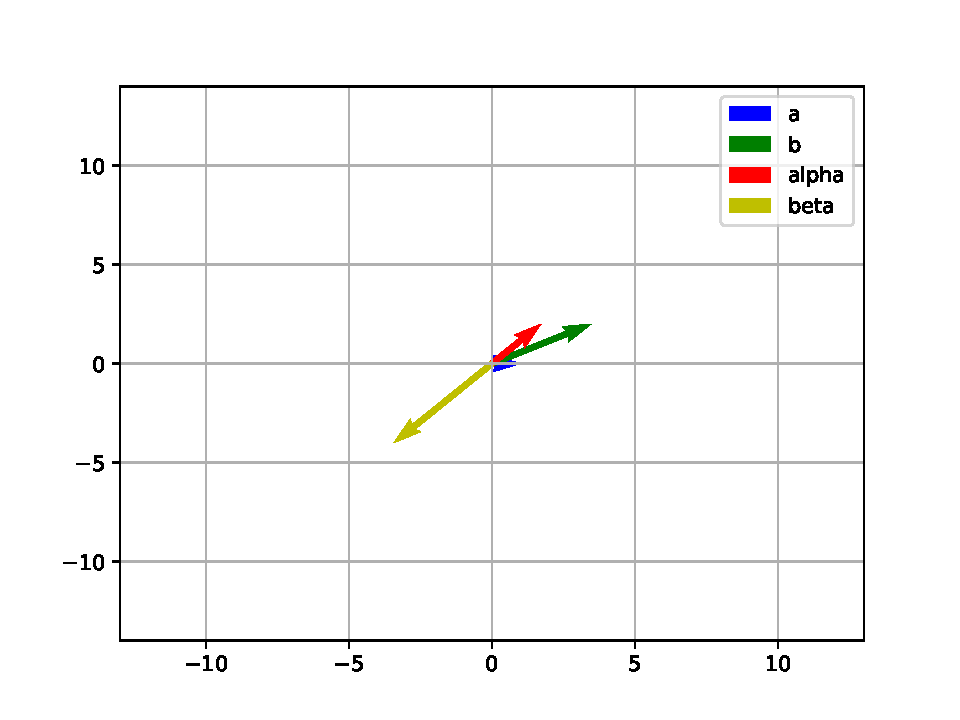
\includegraphics[width=\columnwidth]{figure/fig.pdf}
	\caption{}
	\label{fig:1}
\end{figure}

\end{document}